\documentclass[utf8]{ctexart}
\usepackage{graphicx}
\usepackage{amsmath, amssymb, amsthm}
\usepackage{geometry}
\usepackage{enumitem}
\usepackage{xcolor}
\usepackage{mdframed}
\usepackage{tikz}
\usetikzlibrary{graphs, positioning, arrows.meta}

\geometry{a4paper, margin=2.5cm}

% 定理环境
\newtheoremstyle{mystyle}
  {8pt}{8pt}{\kaishu}{0pt}{\bfseries}{}{1em}{}
\theoremstyle{mystyle}
\newtheorem{theorem}{定理}
\newtheorem{lemma}{引理}

% 好看的题目框
\newmdenv[
  linecolor=black!40,
  linewidth=1pt,
  backgroundcolor=gray!8,
  roundcorner=5pt,
  innertopmargin=8pt,
  innerbottommargin=8pt,
]{problembox}

\title{\textbf{离散数学2\quad 作业1}}
\date{\today}
\author{李子嘉 2024012325}
\begin{document}
\maketitle

\section*{第1题}
\begin{problembox}
\textbf{题目：} 证明：在9座工厂之间，不可能每座工厂都只与其他3座工厂有业务联系，也不可能恰有4座工厂与偶数个工厂有业务联系。
\end{problembox}
\begin{proof}
设9座工厂为无向简单图 $G$ 的9个顶点，工厂之间的业务联系为图中的边。题目等价于：
\begin{itemize}
    \item 不存在一个图 $G$，使得每个顶点的度数都为3。
    \item 不存在一个图 $G$，使得恰有4个顶点的度数为偶数。
\end{itemize}
我们利用图的性质，即图中所有顶点的度数之和等于图中边数的两倍，必须是偶数，来证明这两个结论。

\textbf{第一部分：} 假设存在一个图 $G$，使得每个顶点的度数都为3。则所有顶点的度数之和为 $9 \times 3 = 27$，这是一个奇数，与图的性质矛盾。因此，不存在这样的图。

\textbf{第二部分：} 假设存在一个图 $G$，使得恰有4个顶点的度数为偶数。则剩余的5个顶点的度数为奇数。则所有顶点的度数之和为偶数个偶数加上奇数个奇数，即偶数加上奇数，结果是奇数，与图的性质矛盾。因此，不存在这样的图。
\end{proof}

\section*{第2题}
\begin{problembox}
\textbf{题目：} 简单图 $G$ 有$n$个顶点，$m$条边，如果 $m > \frac{(n-1)(n-2)}{2}$，证明：$G$ 不存在孤立顶点。
\end{problembox}
\begin{proof}
假设 $G$ 存在一个孤立顶点 $v$，则 $v$ 的度数为0。剩余的 $n-1$ 个顶点之间最多有 $\frac{(n-1)(n-2)}{2}$ 条边（完全图 $K_{n-1}$ 的边数）。因此，整个图 $G$ 的边数最多为 $\frac{(n-1)(n-2)}{2}$，与题目中 $m > \frac{(n-1)(n-2)}{2}$ 矛盾。因此，$G$ 不存在孤立顶点。
\end{proof}

\section*{第3题}
\begin{problembox}
\textbf{题目：} 完全图的每边任给一个方向，称为有向完全图。证明在有向完全图中
\[
  \sum_{v_i \in V} \bigl(d^+(v_i)\bigr)^2 = \sum_{v_i \in V} \bigl(d^-(v_i)\bigr)^2.
\]
\end{problembox}

\begin{proof}

设有向完全图共有 $n$ 个顶点。对任意顶点 $v_i$，其出度与入度之和等于其在原完全图中的度数，即
\[
  d^+(v_i) + d^-(v_i) = n - 1. \tag{1}
\]

对所有顶点对 $(1)$ 式求和，注意到每条有向边恰好贡献一次出度和一次入度，故
\[
  \sum_{v_i \in V} d^+(v_i) = \sum_{v_i \in V} d^-(v_i) = \frac{n(n-1)}{2}. \tag{2}
\]

现在考察 $\bigl(d^+(v_i)\bigr)^2 - \bigl(d^-(v_i)\bigr)^2$。利用平方差公式及 $(1)$ 式，得
\[
  \bigl(d^+(v_i)\bigr)^2 - \bigl(d^-(v_i)\bigr)^2
  = \bigl(d^+(v_i) + d^-(v_i)\bigr)\bigl(d^+(v_i) - d^-(v_i)\bigr)
  = (n-1)\bigl(d^+(v_i) - d^-(v_i)\bigr).
\]

对所有顶点求和：
\[
  \sum_{v_i \in V} \Bigl[\bigl(d^+(v_i)\bigr)^2 - \bigl(d^-(v_i)\bigr)^2\Bigr]
  = (n-1) \sum_{v_i \in V} \bigl(d^+(v_i) - d^-(v_i)\bigr)
  = (n-1)\left(\sum_{v_i \in V} d^+(v_i) - \sum_{v_i \in V} d^-(v_i)\right).
\]

由 $(2)$ 式，右端括号内两项相等，故右端为零，即
\[
  \sum_{v_i \in V} \bigl(d^+(v_i)\bigr)^2 - \sum_{v_i \in V} \bigl(d^-(v_i)\bigr)^2 = 0,
\]

从而
\[
  \boxed{\sum_{v_i \in V} \bigl(d^+(v_i)\bigr)^2 = \sum_{v_i \in V} \bigl(d^-(v_i)\bigr)^2.}
\]

\end{proof}

\section*{第4题}
\begin{problembox}
\textbf{题目：} 3个量杯的容量分别是8升、5升和3升，初始时8升量杯装满水，问怎么样才能把水分成两份4升？画出相应的图。
\end{problembox}
\textbf{解：}
将每次倒水后的状态记为三元组 $(a, b, c)$，分别表示8升、5升、3升量杯中的当前水量。
初始状态为 $(8, 0, 0)$，目标状态为 $(4, 4, 0)$。

每次倒水操作将某个量杯倒入另一个量杯，直至来源杯倒空或目标杯装满为止。箭头上标注的 8L$\to$5L 表示将8升量杯中的水倒入5升量杯。
操作如图所示：

\medskip

\begin{center}
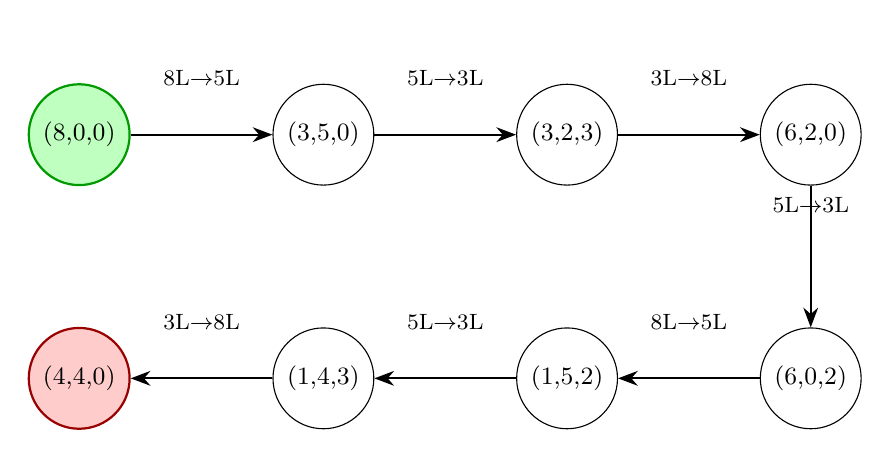
\begin{tikzpicture}[
  node distance=1.8cm,
  every node/.style={circle, draw, minimum size=1.2cm, font=\small},
  start/.style={fill=green!25, draw=green!60!black, thick},
  goal/.style={fill=red!20, draw=red!60!black, thick},
  arr/.style={-{Stealth[length=2.5mm]}, thick},
  lbl/.style={draw=none, fill=none, font=\footnotesize, midway, above=2pt},
]
  \node[start] (s0) {(8,0,0)};
  \node[]      (s1) [right=of s0] {(3,5,0)};
  \node[]      (s2) [right=of s1] {(3,2,3)};
  \node[]      (s3) [right=of s2] {(6,2,0)};
  \node[]      (s4) [below=of s3] {(6,0,2)};
  \node[]      (s5) [left=of  s4] {(1,5,2)};
  \node[]      (s6) [left=of  s5] {(1,4,3)};
  \node[goal]  (s7) [left=of  s6] {(4,4,0)};

  \draw[arr] (s0) -- node[lbl] {8L$\to$5L} (s1);
  \draw[arr] (s1) -- node[lbl] {5L$\to$3L} (s2);
  \draw[arr] (s2) -- node[lbl] {3L$\to$8L} (s3);
  \draw[arr] (s3) -- node[lbl,right=2pt,above=0pt] {5L$\to$3L} (s4);
  \draw[arr] (s4) -- node[lbl] {8L$\to$5L} (s5);
  \draw[arr] (s5) -- node[lbl] {5L$\to$3L} (s6);
  \draw[arr] (s6) -- node[lbl] {3L$\to$8L} (s7);
\end{tikzpicture}
\end{center}

\section*{第5题}

\begin{problembox}
\textbf{题目：} 证明：9个人中若非至少有4个人互相认识，则至少有3个人互相不认识。
\end{problembox}

\begin{proof}

将9个人视为完全图 $K_9$ 的9个顶点，若两人认识则连\textbf{红边}，不认识则连\textbf{蓝边}。
则命题等价于：
\[
  \text{若红色子图不含 } K_4,\quad \text{则蓝色子图含 } K_3.
\]
我们采用\textbf{反证法}：假设蓝色子图也不含 $K_3$（即无3人互相不认识），且红色子图不含 $K_4$（即无4人互相认识），推出矛盾。

\medskip

\textbf{关键引理。}
证明过程中将用到如下两个结论：

\begin{lemma}
$R(3,3) = 6$，即对 $K_6$ 的任意红蓝2-染色，必存在红色 $K_3$ 或蓝色 $K_3$。
\end{lemma}

此引理说明，6个人中，要么至少3个人互相认识，要么至少3个人互相不认识，已在课堂上得到证明。

\begin{lemma}
在上述反证假设下，9人中的每一个人，与其余8人中至多有 $3$ 人不认识（即蓝边数 $b \leq 3$），换言之，每人至少认识其余8人中的 $5$ 人。
\end{lemma}

\begin{proof}[引理2的证明]
任取一人 $v$，设其不认识的人构成集合 $B$，$|B| = b$。
由于蓝色子图不含 $K_3$，$B$ 内任意两人之间不能有蓝边，否则这两人连同 $v$ 将构成蓝色 $K_3$，与假设矛盾。
故 $B$ 内所有边均为红边，即 $B$ 内的人\textbf{两两认识}。
若 $b \geq 4$，则 $B$ 内至少有4人两两认识，构成红色 $K_4$，与反证假设矛盾。
因此 $b \leq 3$，即每人至多与3人不认识。
\end{proof}

\medskip

由引理2，9人中每人的蓝边数 $b \leq 3$，即 $r \geq 5$。任取一人 $v$，记其红色邻居集合为 $R$（$|R|=r$），蓝色邻居集合为 $B$（$|B|=b$）。分情况讨论：

\medskip

\textbf{情况一：$b \leq 2$（即 $r \geq 6$）。}

此时 $v$ 认识至少6个人。由引理1，$R$ 内要么存在红色 $K_3$，要么存在蓝色 $K_3$。由反证假设，$R$ 内不含蓝色 $K_3$，故 $R$ 内必存在红色 $K_3$，设其三个顶点为 $r_1, r_2, r_3$。则 $v, r_1, r_2, r_3$ 四人两两认识，构成红色 $K_4$，矛盾。

\medskip

\textbf{情况二：$b = 3$（即 $r = 5$）。}

由引理2，$b=3$ 是反证假设下 $b$ 能取到的最大值，此情况为情况一之外的唯一剩余情形。
设 $v$ 不认识的3个人为 $b_1, b_2, b_3$，认识的5个人为 $r_1, r_2, r_3, r_4, r_5$。

由引理2的证明，$B = \{b_1, b_2, b_3\}$ 内三人两两认识。

再由引理2，$b_1, b_2, b_3$ 每人至少认识其余8人中的5人。对 $b_i$（$i=1,2,3$）而言，其余8人中，$b_i$ 不认识 $v$，但认识 $B$ 内另外两人，故 $b_i$ 在 $R = \{r_1, r_2, r_3, r_4, r_5\}$ 中至少认识
\[
  5 - 2 = 3 \text{ 人}.
\]

所以，$b_1, b_2, b_3$ 各自在5个 $r_i$ 中至少认识3人，共选至少 $3 \times 3 = 9$ 次（计重数），而 $|R|=5$，由\textbf{鸽巢原理}，至少存在某个 $r_i$ 被 $b_1, b_2, b_3$ \textbf{三人同时认识}。

设此人为 $r_1$，则 $b_1, b_2, b_3, r_1$ 四人中，$b_1, b_2, b_3$ 两两认识且各自认识 $r_1$，故四人两两认识，构成红色 $K_4$，矛盾。

\medskip

\textbf{综上，}
所有$b$的取值均导出矛盾。故反证假设不成立，原命题得证：

\[
  \boxed{\text{若9人中无4人互相认识，则必有3人互相不认识。}}
\]

\end{proof}

\end{document}